\section{Testing Runge-Kutta and Velocity-Verlet for Sun-Earth-Mars System}
\label{sec:SunEarthMarsTest}

\begin{table}[H]
\centering
\caption{Mass, initial position and initial velocity of Sun, Earth and Mars when running the Runge-Kutta 4 algorithm for this three-body problem.
The Earth and Mars are set to orbit in the $x-y$-plane at $z=1$ AU with the distance 1 AU and 1.5 AU to the Sun, respectively, which is not physically true. However, this initialization of position and velocity is reasonable to illustrate the validity of the Runge-Kutta method and Velocity-Verlet method presented in \secref{Newton2body3D}.
}
\begin{center}
\begin{tabular}{ | c | c | c | c |  }
  \hline			
   & mass [$M_{\odot}$] &  $\v{r}_{initial}$ [AU] & $\v{v}_{initial}$ [AU/day]  
  \\ \hline
  Sun & $1.0$ & $(1.0,1.0,1.0)$  & $(0.0,0.0,0.0)$ 
  \\ \hline
  Earth & $3.0\times 10^{-6}$ & $(2.0,1.0,1.0)$ & $(0.0,0.017,0.0)$
  \\ \hline
  Mars & $3.2\times 10^{-7}$ & $(-0.5,1.0,1.0)$  & $(0.0,0.014,0.0)$
  \\ \hline
\end{tabular}
\end{center}
\label{tab:SunEarthMarsTest}
\end{table}

    
\begin{figure}[H]
\centering
\begin{minipage}{.5\textwidth}
  \centering
  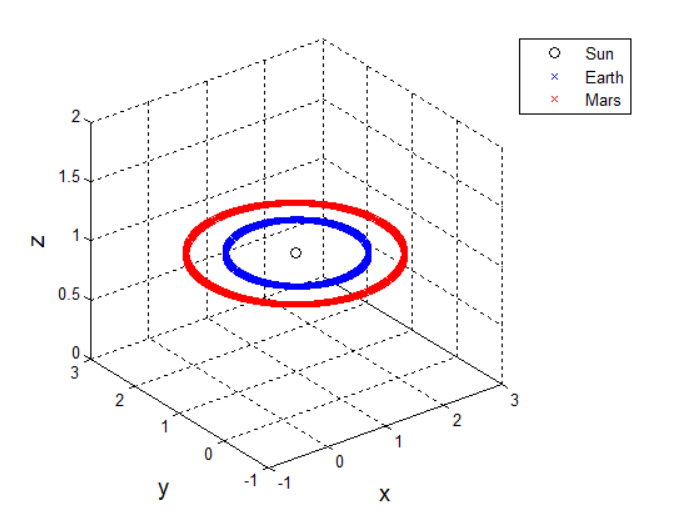
\includegraphics[width=1\linewidth]{Figures/sun_earth_mars_test_RK4.png}
\end{minipage}%
\begin{minipage}{.5\textwidth}
  \centering
  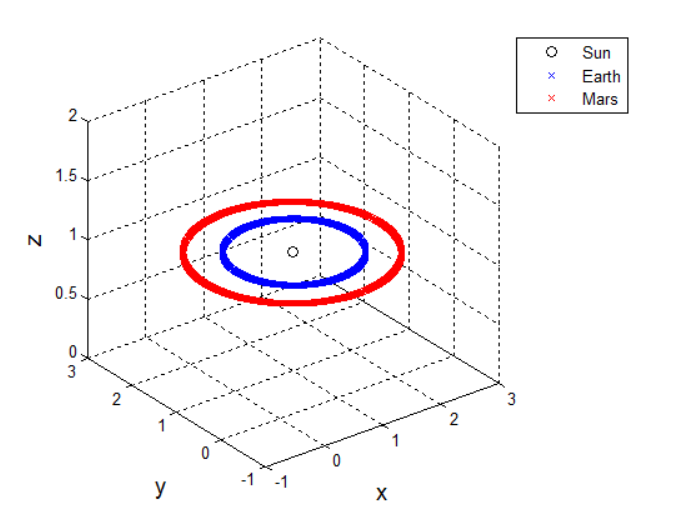
\includegraphics[width=1\linewidth]{Figures/sun_earth_mars_test_VV.png}
\end{minipage}
\caption{
Time evolution of the simplified system of Sun-Earth-Mars over a time period of 20 years using Runge-Kutta (leftmost) and Velocity-Verlet (rightmost) method with a time step length of 1 day.
The masses, initial positions, and initial velocities of the three objects are given in \tabref{tab:SunEarthMarsTest}.
}
\label{fig:SunEarthMarsTest}
\end{figure}

Calculating the initial and final energy of the Sun-Earth-Mars system according to the source code presented en \secref{sec:ComputingEnergy}, gives the following table for different time periods with step length of 1 day.

\begin{table}[H]
\centering
\caption{The final energy after different time periods computed by both the first order Runge-Kutta method and the Velocity-Verlet method for the Sun-Earth-Mars-like system with initial energy of $2.37\times 10^{-9} \text{M}_{\odot} \text{AU}^2 /\text{days}^2$ .
}
\begin{center}
\begin{tabular}{ | c | c | c |  }
  \hline	
  Time period (years) & Final energy (RK4) & Final energy (VV)
  \\ \hline		
  1  & $2.37\times 10^{-9}$ & $2.37\times 10^{-9}$
  \\ \hline
  10  & $2.47\times 10^{-9}$ & $2.47\times 10^{-9}$
  \\ \hline
  100  & $2.50\times 10^{-9}$ & $2.50\times 10^{-9}$
  \\ \hline
  1000 & $2.38\times 10^{-9}$  & $2.38\times 10^{-9}$ 
  \\ \hline
\end{tabular}
\end{center}
\label{tab:SunEarthMarsTest_energy_conservation}
\end{table}
It seems alarming that the final energy if greater than the initial energy for both the fourth order Runge-Kutta method and the Velocity-Verlet method. 
However, with the precision of the constants, e.g. the gravitational constant $G=2.96\times 10^{-4} \text{AU}^3 / \text{days}^2 \cdot \text{M}_{\odot}$, and the time steps, it is conclusive to say that the programmed code for this N-body problem  